%%%%%%%%%%%%%%%%%%%%%%%%%%%%%%%%%%%%%%%%%%%%%%%%%%%%%%%%%%%%%%%%%
%  _____   ____  _____                                          %
% |_   _| /  __||  __ \    Institute of Computitional Physics   %
%   | |  |  /   | |__) |   Zuercher Hochschule Winterthur       %
%   | |  | (    |  ___/    (University of Applied Sciences)     %
%  _| |_ |  \__ | |        8401 Winterthur, Switzerland         %
% |_____| \____||_|                                             %
%%%%%%%%%%%%%%%%%%%%%%%%%%%%%%%%%%%%%%%%%%%%%%%%%%%%%%%%%%%%%%%%%
%
% Project     : LaTeX doc Vorlage für Windows ProTeXt mit TexMakerX
% Title       : 
% File        : doc.tex Rev. 00
% Date        : 23.4.12
% Author      : Remo Ritzmann
% Feedback bitte an Email: remo.ritzmann@pfunzle.ch
%
%%%%%%%%%%%%%%%%%%%%%%%%%%%%%%%%%%%%%%%%%%%%%%%%%%%%%%%%%%%%%%%%%

%%%%%%%%%%%%%%%%%%%%%%%%%%%%%%%%%%%%%%%%%%%%%%%%%%%%%%%%%%%%%%%%%
%  _____   ____  _____                                          %
% |_   _| /  __||  __ \    Institute of Computitional Physics   %
%   | |  |  /   | |__) |   Zuercher Hochschule Winterthur       %
%   | |  | (    |  ___/    (University of Applied Sciences)     %
%  _| |_ |  \__ | |        8401 Winterthur, Switzerland         %
% |_____| \____||_|                                             %
%%%%%%%%%%%%%%%%%%%%%%%%%%%%%%%%%%%%%%%%%%%%%%%%%%%%%%%%%%%%%%%%%
%
% Project     : LaTeX doc Vorlage für Windows ProTeXt mit TexMakerX
% Title       : 
% File        : header.tex Rev. 00
% Date        : 23.4.12
% Author      : Remo Ritzmann
% Feedback bitte an Email: remo.ritzmann@pfunzle.ch
%
%%%%%%%%%%%%%%%%%%%%%%%%%%%%%%%%%%%%%%%%%%%%%%%%%%%%%%%%%%%%%%%%%

\documentclass[
	oneside,
	10pt,
	parskip=half,
	ngerman,
	%bibtotocnumbered,
	%bibliography=totocnumbered,
	listof=totoc,
	version=first
	%liststotoc
]{scrreprt}
%article scrartcl
%report scrreprt
%book scrbook
%letter scrlttr2

%***********************************************************************
% include some libs
%***********************************************************************	
\usepackage[utf8]{inputenc}
\usepackage{listings}
\usepackage{color}
\usepackage{fancyhdr}
\usepackage{rotating}
\usepackage{titlesec}
\usepackage{mathptmx} 
\usepackage[scaled=.90]{helvet}
%\usepackage{times}
%\renewcommand*\familydefault{\sfdefault} %% Only if the base font of the document is to be sans serif
\usepackage[T1]{fontenc}
\usepackage{german}
%\usepackage[ngerman]{babel}
%\usepackage[babel]{csquotes}
\usepackage{textcomp}
\usepackage[squaren]{SIunits}
\usepackage{graphicx}
\usepackage{url}
\usepackage{geometry}
\usepackage[absolute]{textpos}
\usepackage{makeidx}
\usepackage{colortbl}
\usepackage{pdflscape}
\usepackage{pdfpages}
\usepackage{tabularx}
\usepackage{lmodern}
\usepackage{longtable}
\usepackage{array}
\usepackage{float}
\usepackage{scrhack}
\usepackage{wallpaper}
\usepackage{titleref}

% Bereitstellung Hyperlinkfunktionen (PDF) (muss als letztes Paket geladen werden)
\usepackage[
	colorlinks=true,
	breaklinks=true,
	linkcolor=black,
	citecolor=black,
	urlcolor=black,
	anchorcolor=black,
	pdfpagelabels,
	pdftitle={Seminararbeit},
	pdfsubject={Facebook und der Glücksfaktor},
	pdfkeywords={KEYWORDS},
	pdfauthor={Till J. Ernst (ernsttil)}
]{hyperref}

\usepackage{apacite}

% biblatex-apa
%\usepackage[style=apa,
%			backend=biber,
%			babel=hyphen,
%			natbib=true
%			style=authoryear, 
%    		maxcitenames=2, 
%    		sorting=nyt,
%    		backref=true
%]{biblatex}
%\DeclareLanguageMapping{ngerman}{{ngerman-apa}} 
%\addbibresource{Literatur} %for biblatex


% Bereitstellung Glossar
\usepackage[toc]{glossaries}
\makeglossaries



%***********************************************************************
% various styles
%***********************************************************************	

%create index
\makeindex

%define pagestyle
\pagestyle{fancy}

%use sans-serif font 
%\renewcommand{\familydefault}{\sfdefault}

%define page margin
\geometry{a4paper, top=25mm, left=25mm, right=25mm, bottom=25mm,headsep=10mm,footskip=10mm}

%textpos parameter
\setlength{\TPHorizModule}{30mm}
\setlength{\TPVertModule}{\TPHorizModule}
\textblockorigin{10mm}{10mm} % start everything near the top-left corner
\setlength{\parindent}{0pt}

%horizontal lines for titlepage 
\newcommand{\HRule}{\rule{\linewidth}{0.5mm}}

%reference to source items inlc source number
\newcommand{\srcref}[1]{\nameref{src:#1} \cite{#1}}

%header / footer 
\renewcommand{\headrulewidth}{0.3pt}
\renewcommand{\footrulewidth}{0.3pt}

\fancyhead[LO,RE]{} %clear headings for contents 
\fancyhead[RO,LE]{\nouppercase{\rightmark}} %right odd pages and left even pages
\fancyhead[LO,RE]{\MakeUppercase{\leftmark}} %left odd pages and right even pages
\fancyfoot[LE,RO]{\thepage} %page numbering
\fancyfoot[C]{} %clear centered page numbering 

%define some colors
\definecolor{gray}{rgb}{0.95,0.95,0.95}
\definecolor{darkgray}{rgb}{0.4,0.4,0.4}
%listing colors
\definecolor{lgray}{RGB}{250,250,250}
\definecolor{lgreen}{RGB}{63,127,95}
\definecolor{lred}{RGB}{127,0,85}
\definecolor{lblue}{RGB}{42,0,255}

%***********************************************************************
% listing
%***********************************************************************

\lstset{		
		basicstyle=\small\ttfamily,
		frame=single,
		numbers=left,	
		numberstyle=\tiny,
		%firstnumber=auto,
		numberblanklines=true,
		captionpos=b,
		extendedchars=true,
		float=ht,
		showtabs=false,
		tabsize=2,
		showspaces=false,
		showstringspaces=false,
		breaklines=true,
		%prebreak=\Righttorque,
		backgroundcolor=\color{lgray},
		keywordstyle=\color{lred}\bfseries, 
		commentstyle=\color{lgreen}\ttfamily,
%		morekeywords={printstr, printhexln},
		stringstyle=\color{lblue},
		xleftmargin=0.5cm,
		xrightmargin=0.5cm
}

%\lstloadlanguages{C++}

%\lstdefinelanguage{xc}{
%     keywords={printstr, printhexln, attributes, class, classend, do, empty, endif, endwhile, fail, function, functionend, if, implements, in, inherit, inout, not, of, operations, out, return, set, then, types, while, use},
%     keywordstyle=\color{lred}\bfseries,
%     ndkeywords={},
%     ndkeywordstyle=\color{yellow}\bfseries,
%     identifierstyle=\color{black},
%     sensitive=false,
%     comment=[l]{//},
%     commentstyle=\color{lgreen}\ttfamily,
%     string=[l]{"},
%     stringstyle=\color{lblue}\ttfamily
%  }


\begin{document}
\title{PA/BA Latex Vorlage}
\author{Remo Ritzmann}


%%%%%%%%%%%%%%%%%%%%%%%%%%%%%%%%%%%%%%%%%%%%%%%%%%%%%%%%%%%%%%%%%
%  _____   ____  _____                                          %
% |_   _| /  __||  __ \    Institute of Computitional Physics   %
%   | |  |  /   | |__) |   Zuercher Hochschule Winterthur       %
%   | |  | (    |  ___/    (University of Applied Sciences)     %
%  _| |_ |  \__ | |        8401 Winterthur, Switzerland         %
% |_____| \____||_|                                             %
%%%%%%%%%%%%%%%%%%%%%%%%%%%%%%%%%%%%%%%%%%%%%%%%%%%%%%%%%%%%%%%%%
%
% Project     : LaTeX doc Vorlage für Windows ProTeXt mit TexMakerX
% Title       : 
% File        : titlepage.tex Rev. 01
% Date        : 23.4.12
% Author      : Remo Ritzmann
% Feedback bitte an Email: remo.ritzmann@pfunzle.ch
%
%%%%%%%%%%%%%%%%%%%%%%%%%%%%%%%%%%%%%%%%%%%%%%%%%%%%%%%%%%%%%%%%%

\begin{titlepage}

% Logo
\ThisTileWallPaper{\paperwidth}{\paperheight}{images/logos/InIT.pdf} % {}images/logos/*.pdf}
% Wählen Sie aus folenden pdf Files: ICP, IDP, IEFE, IMES, IMPE, IMS, INE, InES, InIT, KSR, SoE, ZAMP, ZAV, ZIL, ZPP, ZSN

\begin{minipage}[b]{0.117\textwidth}
\hskip 0.05cm
\end{minipage}
\begin{minipage}[b]{0.91\textwidth}
\begin{tiny}.\end{tiny}\vskip 2.8cm
	{\huge
	
	% Projekt Name
	\textbf{\underline{Bachelor-/Projektarbeit (Studiengang)}}\\
	\textbf{\underline{max. 2 Zeilen}}
	
	% Projekt Titel
	Titel der Arbeit Titel der Arbeit Titel der Arbeit Titel der Arbeit Titel der Arbeit Titel der Arbeit Titel der Arbeit Titel der Arbeit Titel der Arbeit Titel der (max. 4 Zeilen)
	\vskip 0.5cm}
	
	\begin{minipage}[b]{0.27\textwidth}
	\hrule\vskip 0.5cm
		\textbf{Autoren}\\
		\\
	\end{minipage}
	\begin{minipage}[b]{0.03\textwidth}
	\hskip 0.5cm
	\end{minipage}
	\begin{minipage}[b]{0.7\textwidth}
	\hrule\vskip 0.5cm
		Vorname Name\\
		Vorname Name\\
	\end{minipage}
	
	\begin{minipage}[b]{0.27\textwidth}
	\hrule\vskip 0.5cm
		\textbf{Hauptbetreuung}\\
		\\
	\end{minipage}
	\begin{minipage}[b]{0.03\textwidth}
	\hskip 0.5cm
	\end{minipage}
	\begin{minipage}[b]{0.7\textwidth}
	\hrule\vskip 0.5cm
		Vorname Name\\
		Vorname Name\\
	\end{minipage}
	
	\begin{minipage}[b]{0.27\textwidth}
	\hrule\vskip 0.5cm
		\textbf{Nebenbetreuung}\\
		\\
	\end{minipage}
	\begin{minipage}[b]{0.03\textwidth}
	\hskip 0.5cm
	\end{minipage}
	\begin{minipage}[b]{0.7\textwidth}
	\hrule\vskip 0.5cm
		Vorname Name\\
		Vorname Name\\
	\end{minipage}
	
	\begin{minipage}[b]{0.27\textwidth}
	\hrule\vskip 0.5cm
		\textbf{Industriepartner}\\
		\\
	\end{minipage}
	\begin{minipage}[b]{0.03\textwidth}
	\hskip 0.5cm
	\end{minipage}
	\begin{minipage}[b]{0.7\textwidth}
	\hrule\vskip 0.5cm
		Firmenname\\
		\\
	\end{minipage}
	
	\begin{minipage}[b]{0.27\textwidth}
	\hrule\vskip 0.5cm
		\textbf{Externe Betreuung}\\
		\\
	\end{minipage}
	\begin{minipage}[b]{0.03\textwidth}
	\hskip 0.5cm
	\end{minipage}
	\begin{minipage}[b]{0.7\textwidth}
	\hrule\vskip 0.5cm
		Vorname Name\\
		Vorname Name\\
	\end{minipage}
	
	\begin{minipage}[b]{0.27\textwidth}
	\hrule\vskip 0.5cm
		\textbf{Datum}
	\end{minipage}
	\begin{minipage}[b]{0.03\textwidth}
	\hskip 0.5cm
	\end{minipage}
	\begin{minipage}[b]{0.7\textwidth}
	\hrule\vskip 0.5cm
		01.01.2011
	\end{minipage}
\end{minipage}
\vskip 0.5cm

\textcolor{darkgray}{
Bitte füllen Sie das Titelblatt aus und berücksichtigen Sie Folgendes:\\
 -> Bitte auf keinen Fall Schriftart und Schriftgrösse ändern. Text soll lediglich überschrieben werden!\\
 -> Bitte pro Tabellenzeile max. 4 Textzeilen!\\
\\
•	Vorlage: Haben Sie die richtige Vorlage gewählt? Logo Institut/Zentrum\\
•	Titel: Fügen Sie Ihren Studiengang direkt nach dem Wort „Bachelorarbeit“ ein (max. 2 Zeilen).\\
•	Titel der Arbeit: Überschreiben Sie den Lauftext mit dem Titel Ihrer Arbeit (max. 4 Zeilen).\\
•	Autoren: Tragen Sie Ihre Vor- und Nachnamen ein (alphabetisch nach Name).\\
•	Betreuer: Tragen Sie Ihren Betreuer / Ihre Betreuer ein (alphabetisch nach Name).\\
•	Ohne Nebenbetreuung, Industriepartner oder externe Betreuung, ganze Tabellenzeile löschen.\\
•	Datum: Aktuelles Datum eintragen.\\
•	Am Schluss löschen Sie den ganzen Beschrieb (grau) und speichern das Dokument als pdf. ab.
}

\end{titlepage}


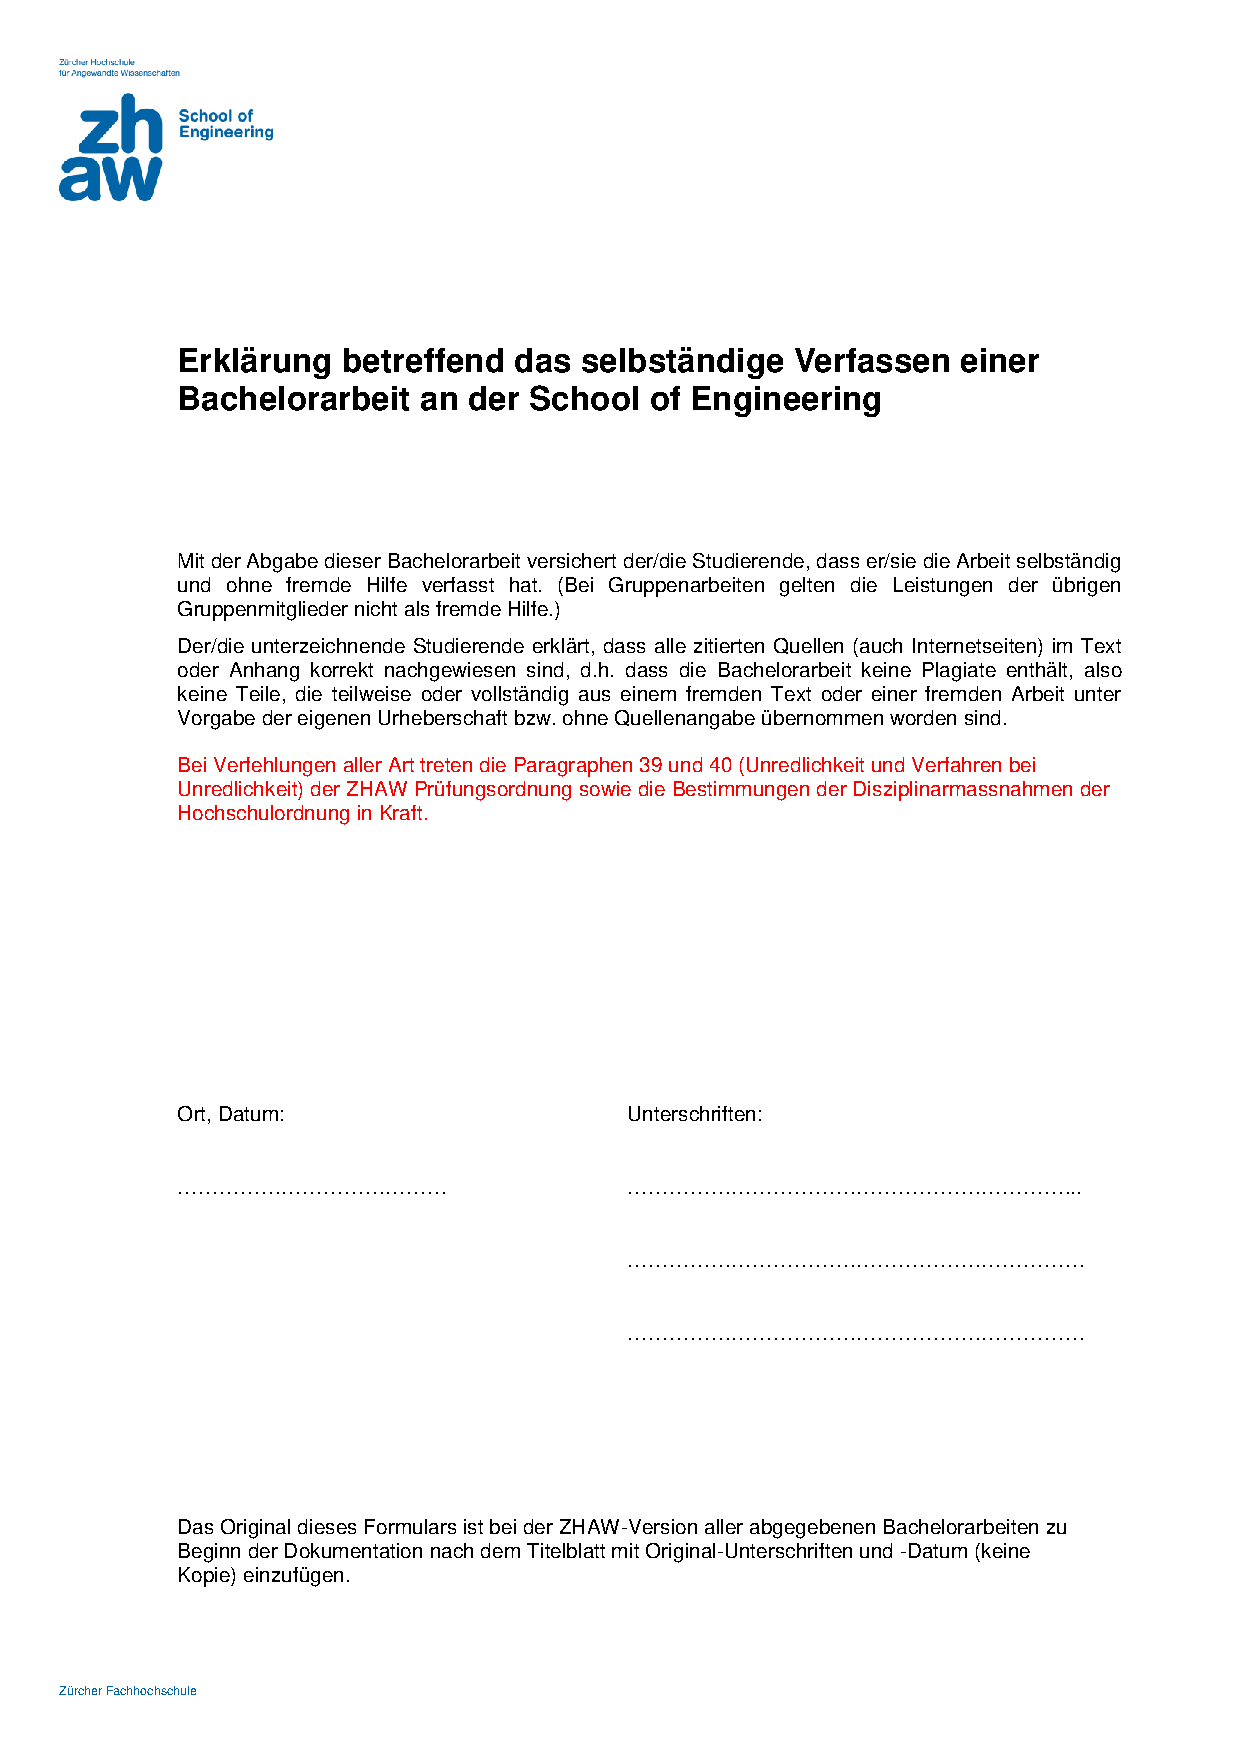
\includepdf{images/Erklaerung_BA.pdf} % Entsprechendes auskommentieren
% 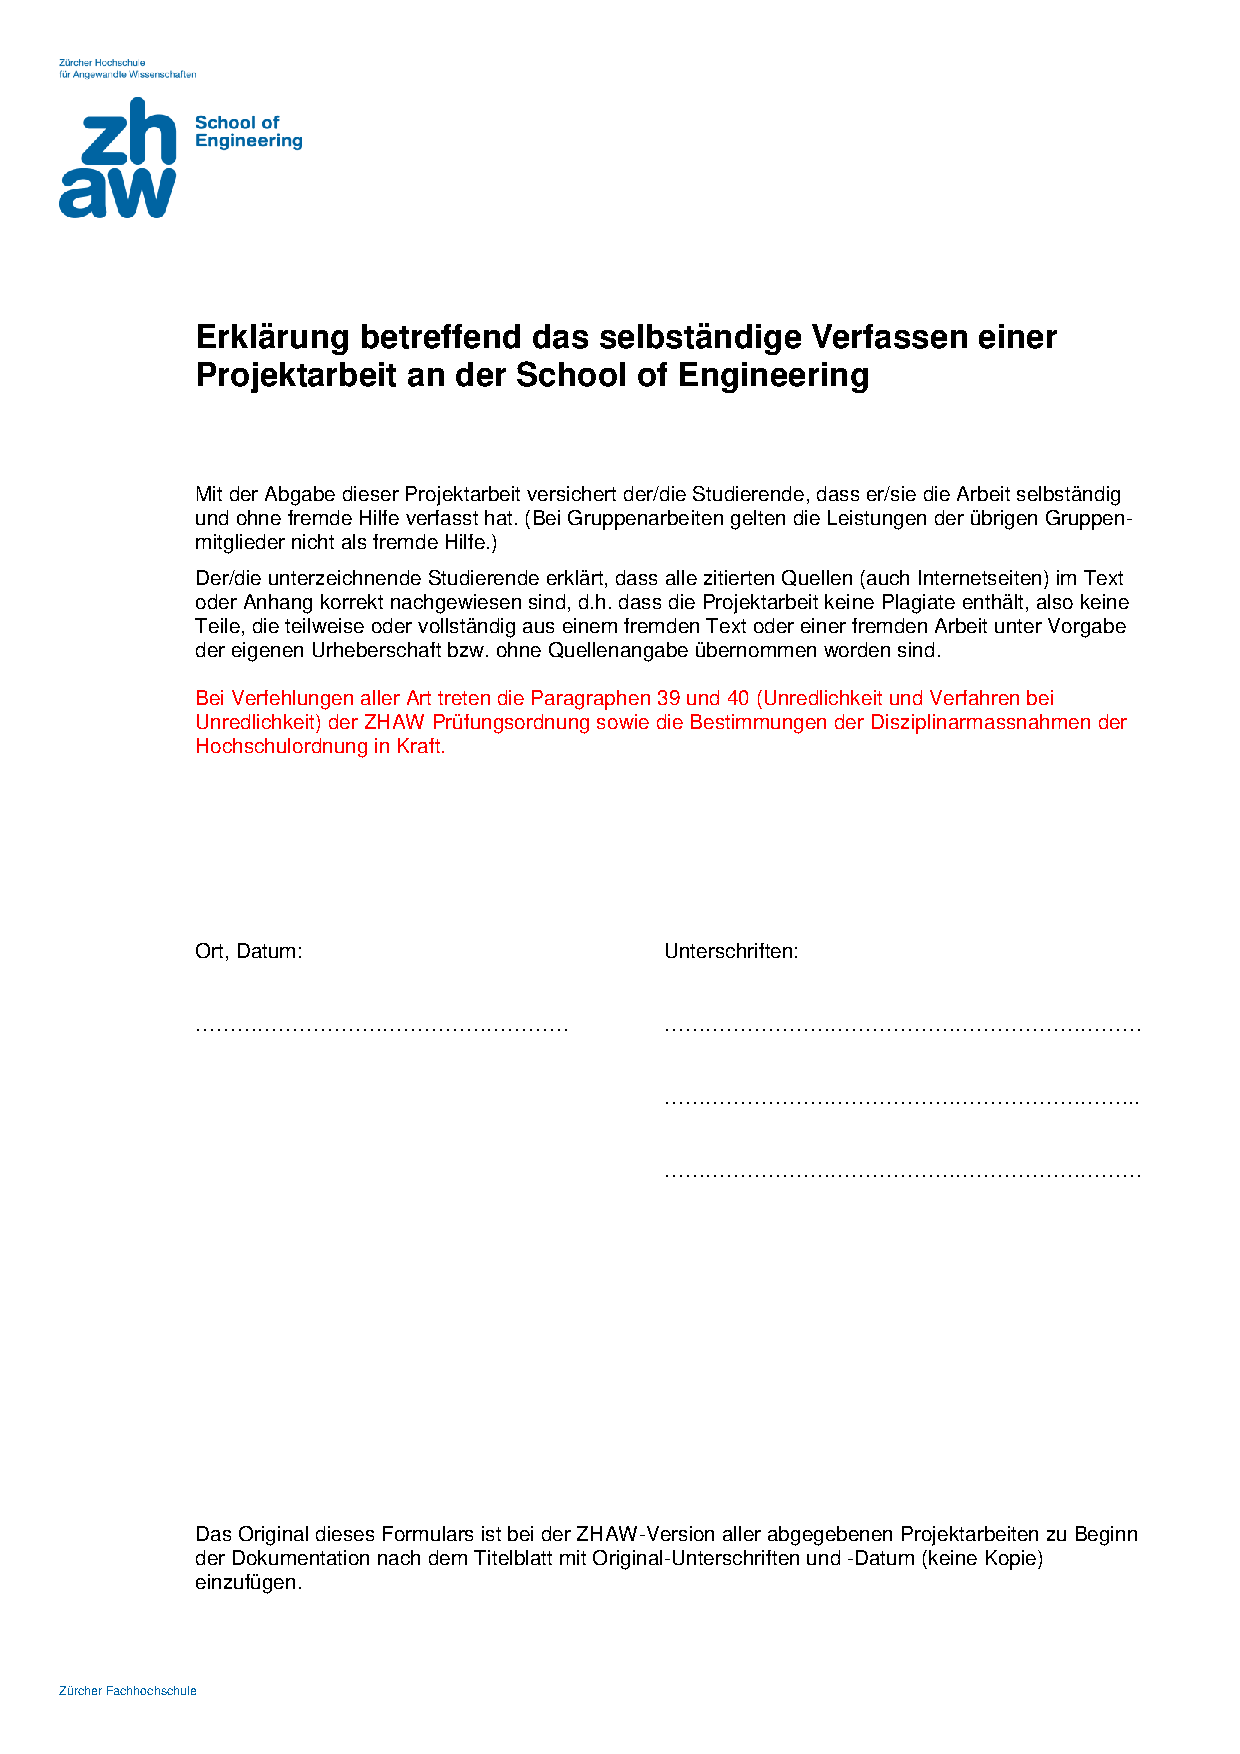
\includepdf{images/Erklaerung_PA.pdf}

\setcounter{page}{1}
%%%%%%%%%%%%%%%%%%%%%%%%%%%%%%%%%%%%%%%%%%%%%%%%%%%%%%%%%%%%%%%%%%
%  _____   ____  _____                                          %
% |_   _| /  __||  __ \    Institute of Computitional Physics   %
%   | |  |  /   | |__) |   Zuercher Hochschule Winterthur       %
%   | |  | (    |  ___/    (University of Applied Sciences)     %
%  _| |_ |  \__ | |        8401 Winterthur, Switzerland         %
% |_____| \____||_|                                             %
%%%%%%%%%%%%%%%%%%%%%%%%%%%%%%%%%%%%%%%%%%%%%%%%%%%%%%%%%%%%%%%%%
%
% Project     : LaTeX doc Vorlage für Windows ProTeXt mit TexMakerX
% Title       : 
% File        : Kontakt.tex Rev. 00
% Date        : 23.4.12
% Author      : Remo Ritzmann
% Feedback bitte an Email: remo.ritzmann@pfunzle.ch
%
%%%%%%%%%%%%%%%%%%%%%%%%%%%%%%%%%%%%%%%%%%%%%%%%%%%%%%%%%%%%%%%%%

\textbf{Kontakte}


\textbf{Vorlagen Ersteller} \\
M.Sc. Engineering ZHAW Remo Ritzmann \\
Wissenschaftliche Assistent Optoelectronic Research Laboratory\\
School of Engineering\\
Technikumstrasse 9, TL419\\
CH-8408 Winterthur

Phone: +41 (0)52 534 48 62\\
Zentrale: +41 (0)58 934 73 06\\
Mobile: +41 (0)79 830 17 35\\
E-Mail: remo.ritzmann@zhaw.ch\\
E-Mail Privat: remo.ritzmann@pfunzle.ch\\
Homepage: \url{http://www.icp.zhaw.ch}\vskip 15pt

%%%%%%%%%%%%%%%%%%%%%%%%%%%%%%%%%%%%%%%%%%%%%%%%%%%%%%%%%%%%%%%%%
%  _____   ____  _____                                          %
% |_   _| /  __||  __ \    Institute of Computitional Physics   %
%   | |  |  /   | |__) |   Zuercher Hochschule Winterthur       %
%   | |  | (    |  ___/    (University of Applied Sciences)     %
%  _| |_ |  \__ | |        8401 Winterthur, Switzerland         %
% |_____| \____||_|                                             %
%%%%%%%%%%%%%%%%%%%%%%%%%%%%%%%%%%%%%%%%%%%%%%%%%%%%%%%%%%%%%%%%%
%
% Project     : LaTeX doc Vorlage für Windows ProTeXt mit TexMakerX
% Title       : 
% File        : abstract.tex Rev. 00
% Date        : 23.4.12
% Author      : Remo Ritzmann
% Feedback bitte an Email: remo.ritzmann@pfunzle.ch
%
%%%%%%%%%%%%%%%%%%%%%%%%%%%%%%%%%%%%%%%%%%%%%%%%%%%%%%%%%%%%%%%%%

\thispagestyle{empty}
\chapter*{Zusammenfassung}\label{chap.zusammenfassung}
Zusammenfassung in Deutsch



\newpage
\thispagestyle{empty}
\chapter*{Abstract}\label{abstract}
Abstract in English



\chapter*{(Deutschsprachiges Management Summary)}\label{ManagementSummaryDE}



\chapter*{(Englischsprachiges Management Summary)}\label{ManagementSummaryEN}



\chapter*{Vorwort}\label{vorwort}
Stellt den persönlichen Bezug zur Arbeit dar und spricht Dank aus.


%Inhaltsverzeichnis
\tableofcontents
\newpage


%Kapitel
%\setcounter{page}{1}
%\pagenumbering{arabic}

%%%%%%%%%%%%%%%%%%%%%%%%%%%%%%%%%%%%%%%%%%%%%%%%%%%%%%%%%%%%%%%%%
%  _____   ____  _____                                          %
% |_   _| /  __||  __ \    Institute of Computitional Physics   %
%   | |  |  /   | |__) |   Zuercher Hochschule Winterthur       %
%   | |  | (    |  ___/    (University of Applied Sciences)     %
%  _| |_ |  \__ | |        8401 Winterthur, Switzerland         %
% |_____| \____||_|                                             %
%%%%%%%%%%%%%%%%%%%%%%%%%%%%%%%%%%%%%%%%%%%%%%%%%%%%%%%%%%%%%%%%%
%
% Project     : LaTeX doc Vorlage für Windows ProTeXt mit TexMakerX
% Title       : 
% File        : header.tex Rev. 00
% Date        : 23.4.12
% Author      : Remo Ritzmann
% Feedback bitte an Email: remo.ritzmann@pfunzle.ch
%
%%%%%%%%%%%%%%%%%%%%%%%%%%%%%%%%%%%%%%%%%%%%%%%%%%%%%%%%%%%%%%%%%

\chapter{LaTeX Kurzanleitung}\label{chap.anleitung}
Dieses Kapitel führt mit Beispielcode in den LaTeX Code ein.\footnote{Verbesserungsvorschläge bitte an remo.ritzmann@pfunzle.ch senden}

Die nachfolgende Berichtstruktur wurde aus der Vorlage\footnote{Berichtstruktur Vorlage, Stand: August 2011} der \href{https://intra.zhaw.ch/departemente/school-of-engineering/studium-standort-winterthur/studierende/projektarbeit-bachelorarbeit.html}{PA/BA Termin-Webseite} vom ZHAW Intranet entnommen.

(): alle in Klammer aufgeführten Einträge sind situativ anzupassen



\section{Visio Vektorgraphik einfügen}\label{visio}
(Graphik auswählen) Speichern unter -> PDF -> Optionen.. -> Auswahl\\
Mit Adobe Akrobat öffnen: Erweitert -> Druckproduktion -> Seiten beschneiden -> Weisse Ränder entfernen -> OK -> Ctrl-S

\begin{figure}[H]
	\centering
		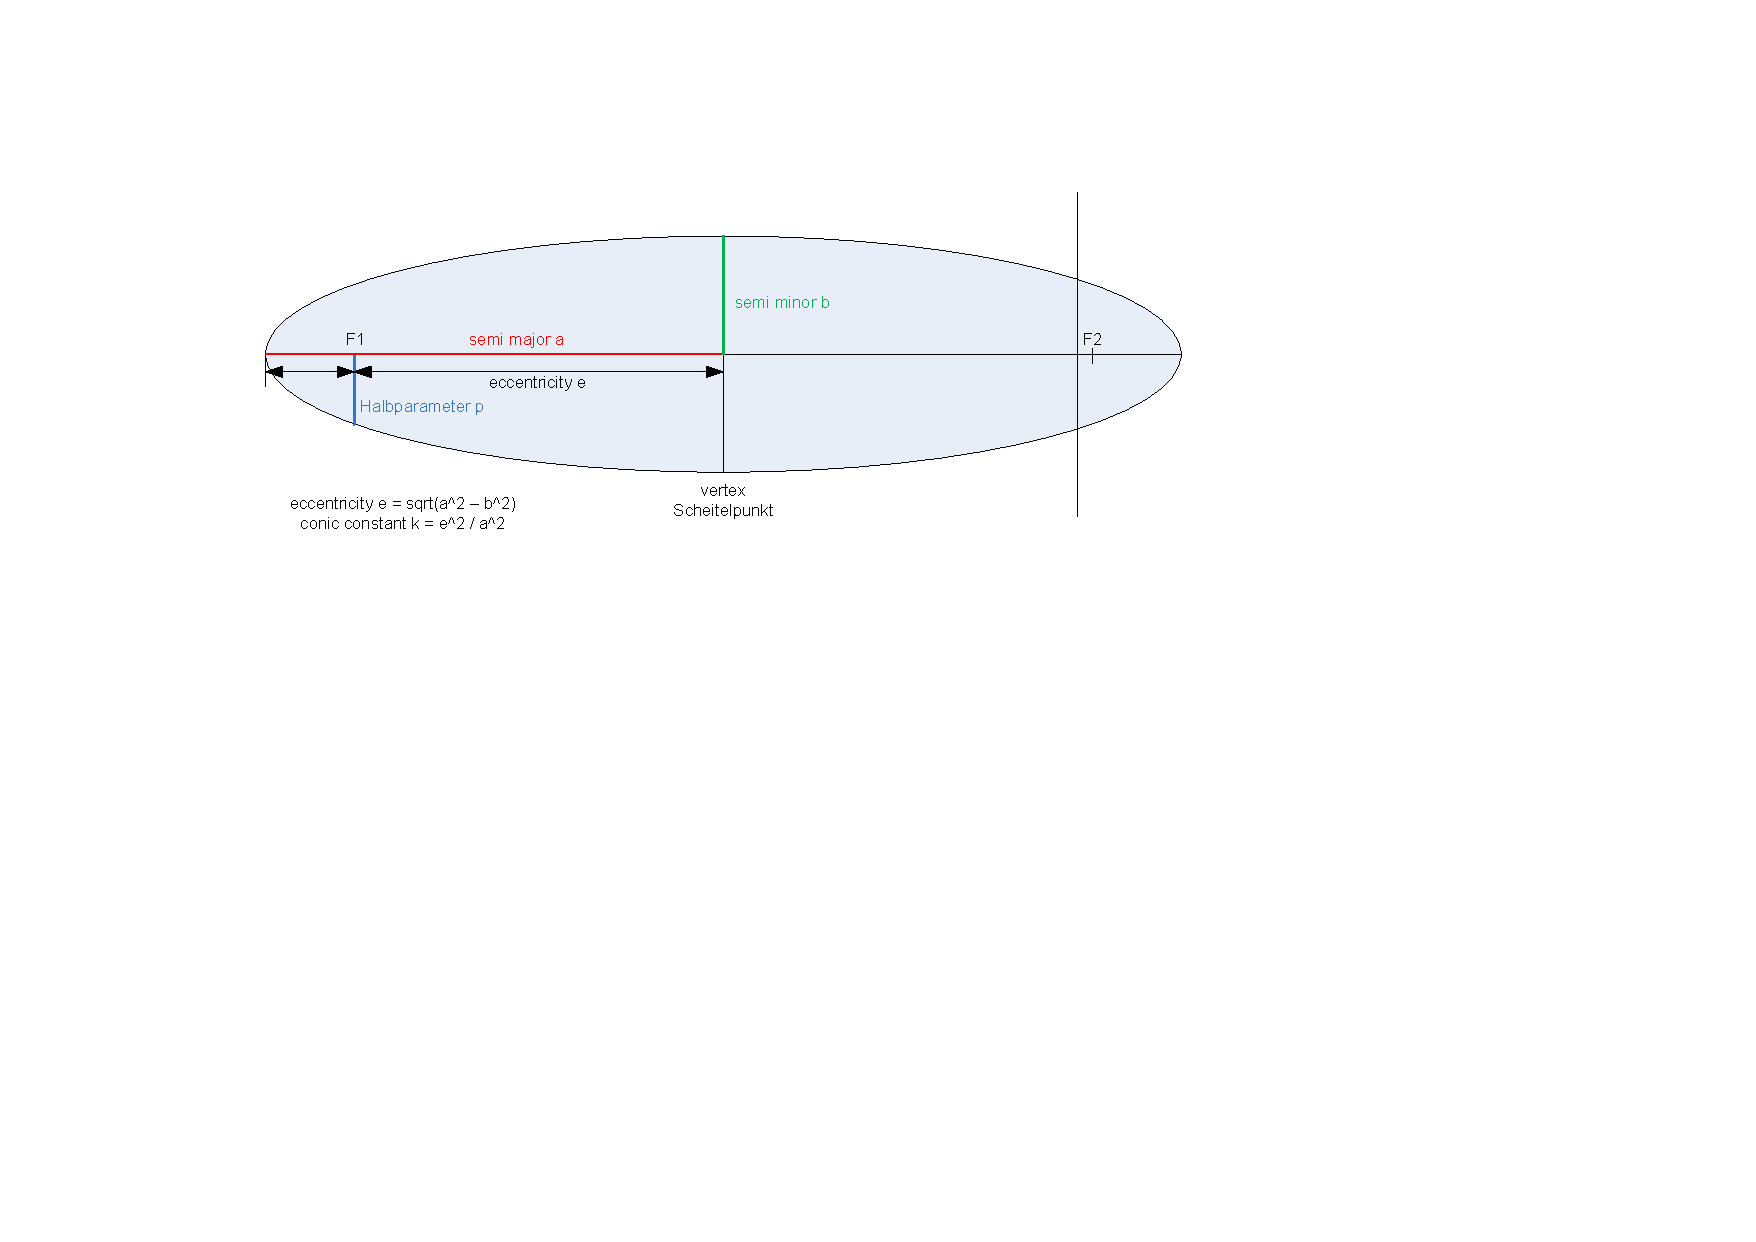
\includegraphics[width=0.8\textwidth]{images/visio/visio.pdf}
	\caption{Ideenskizze}
	\label{fig.Skizze}
\end{figure}

So kann die Abbildung~\ref{fig.Skizze} referenziert werden. Bei der PDF Erstellung ist darauf zu achten, dass LaTeX nur Versionen bis 1.4 voll unterstützt. 



\subsection{Graphiken in LaTeX zuschneiden}\label{zuschneiden}
Mit dem Befehl Clip kann eine Graphik auch in LaTeX zugeschnittenwerden:

\begin{figure}[H]
	\centering
		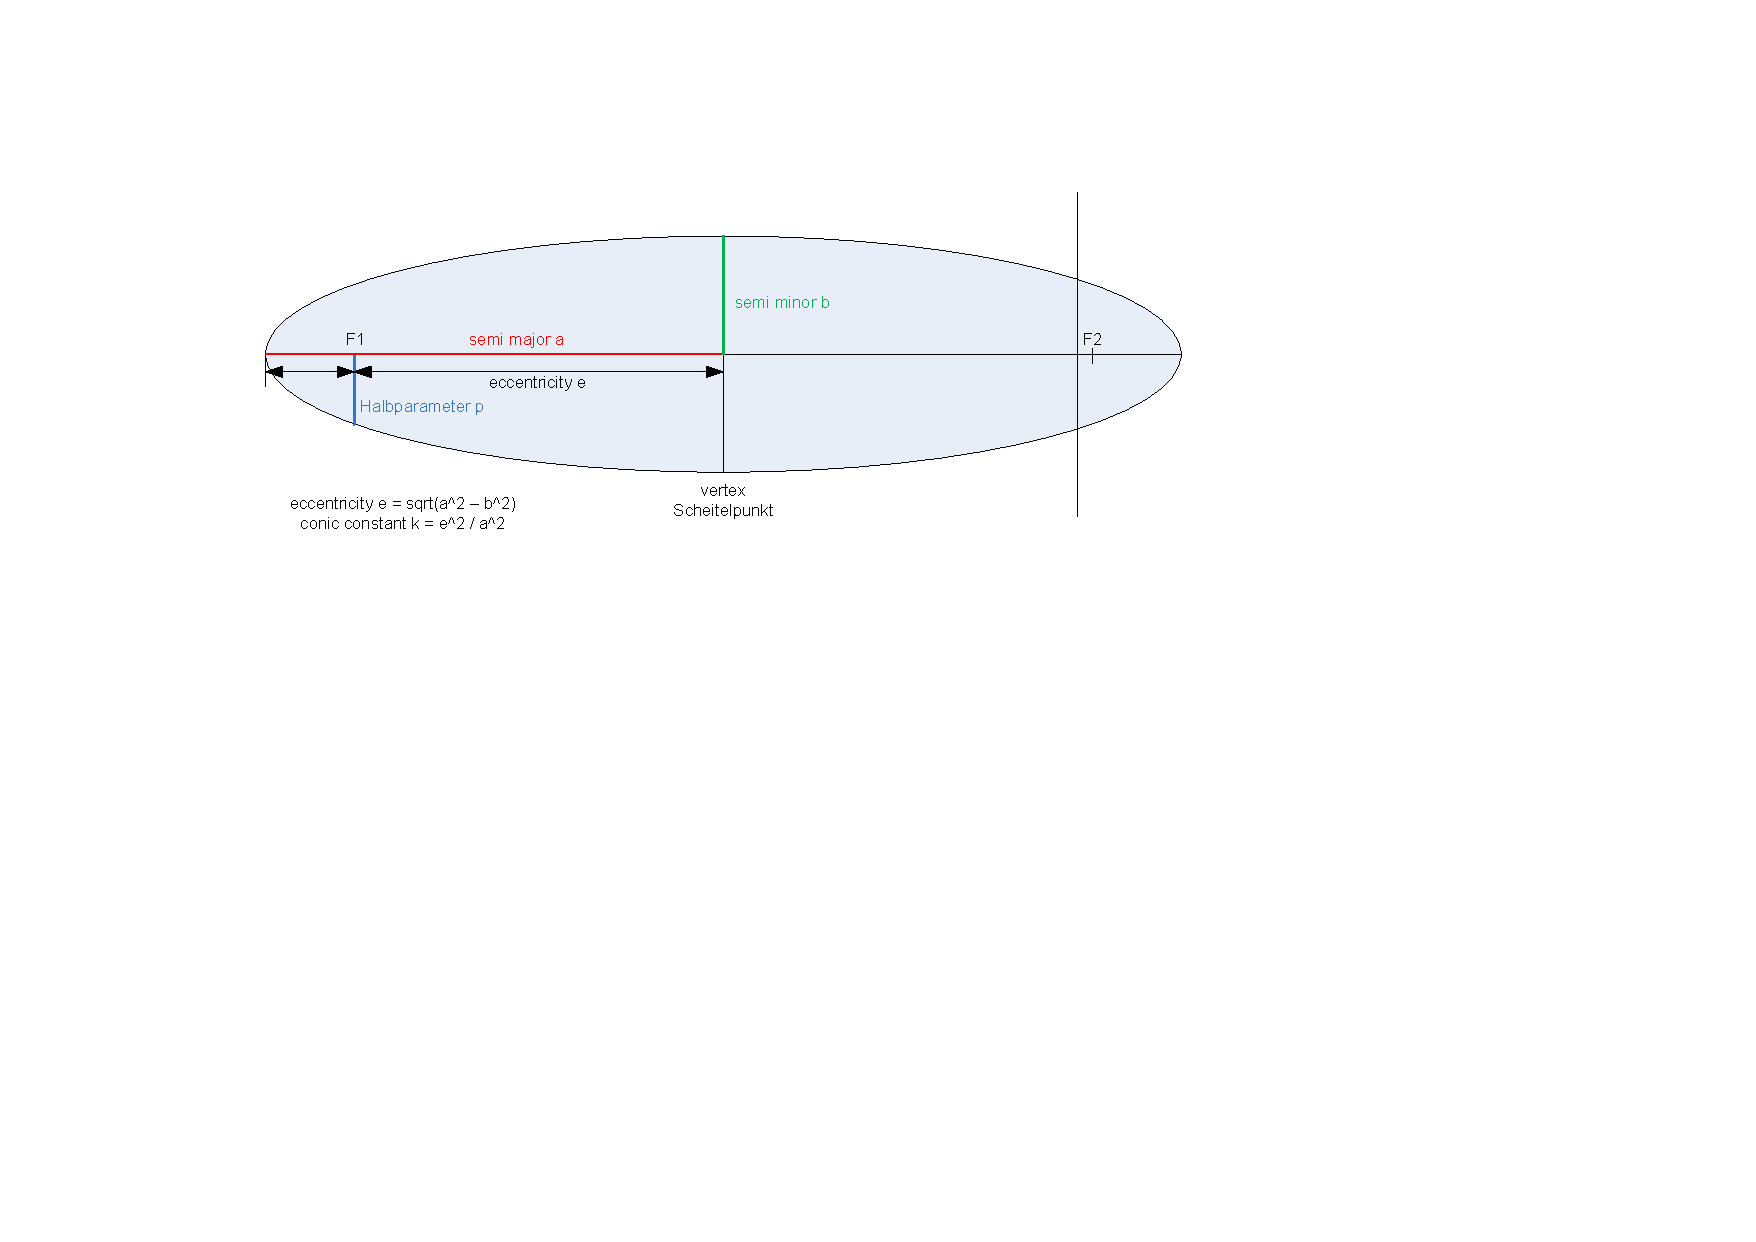
\includegraphics[width=0.9\textwidth, clip=true, trim = 80 10 0 10]{images/visio/visio.pdf}  % trim lm bm rm tm (left, bottom, right, top)
	\caption{clip=true, trim = 60 10 0 10}
	\label{fig.SkizzeZugeschnitten}
\end{figure}




\subsection{Mehrere Bilder nebeneinander}\label{nebeneinander}
Dank Minipages können mehrere Bilder auch nebeneinander sein:

%Zwei Bilder nebeneinander http://latex.mschroeder.net/
\begin{figure}[H]
  \centering
  \begin{minipage}[b]{0.45\textwidth}
    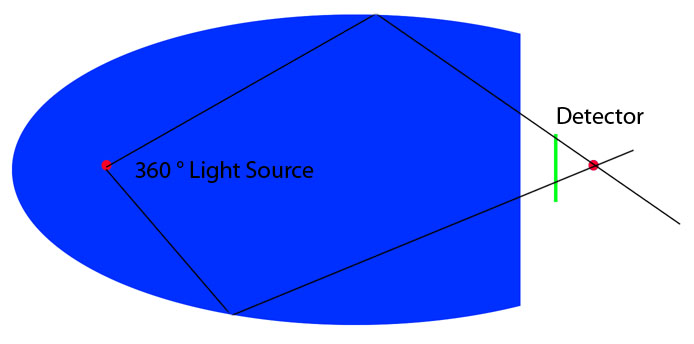
\includegraphics[scale=0.15]{images/photoshop/Skizze.jpg}
    \caption{Visir10b Detector}
    \label{Visir10bDetector} 
  \end{minipage} % Hier darf keine Leerzeile zwischen den beiden Minipages liegen!
  \begin{minipage}[b]{0.45\textwidth}
    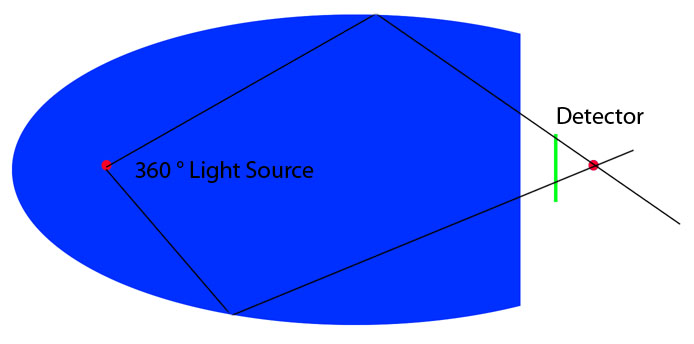
\includegraphics[scale=0.15]{images/photoshop/Skizze.jpg} 
    \caption{Visir10b Model}
    \label{Visir10bModel} 
  \end{minipage}
  \caption{Visir 10 mit optimiertem Reflektor}
  \label{fig.Visir10b}
\end{figure}


\section{Tabellen aufbauen}\label{tabelle}
Kleine Tabelle:

\begin{table}[ht] \centering
	\begin{tabular}{|p{3cm}|p{.5cm}|p{.5cm}|p{.5cm}|p{.5cm}|p{.5cm}|p{.5cm}|p{.5cm}|p{.5cm}|p{.5cm}|p{.5cm}|} \hline
		\rowcolor{gray} Modul & M01 & M02 & M03 & M04 & M05 & M06 & M07 & M08 & M09 & M10 \\
		\hline
		FPGA\_DATEN & & & & & X & X & & X & X & \\
		\hline
		IRQ & X & X & X & & X & & & & X & X \\
		\hline
		Nachbar Core & & & & X & & X & & X & & \\
		\hline
	\end{tabular}
	\caption{Port Schwierigkeiten der Funkmodule}
	\label{tab:portprobleme}
 \end{table}	

Die nachfolgende longtable kann sich über mehrere Seiten erstrecken.

\begin{longtable}{|p{1.1cm}|p{4cm}|p{4cm}|p{4cm}|} 
					\hline
					\rowcolor{gray} Typ & Variante A & Variante B & Variante C
					\\ \hline
					& \textbf{Vorteile:} 
							\begin{itemize}
								\item[+] hohe Spannungen
							\end{itemize}							
							\textbf{Nachteile:}
							\begin{itemize}
								\item[-] Grosse Abmessung
							\end{itemize}
					& 	\textbf{Vorteile:} 
							\begin{itemize}
								\item[+] einfache Montage
							\end{itemize}							
							\textbf{Nachteile:}
							\begin{itemize}
								\item[-] max. 2A Eingangsstrom
							\end{itemize}
					&	\textbf{Vorteile:} 
							\begin{itemize}
								\item[+] hoher Strom
							\end{itemize}							
							\textbf{Nachteile:}
							\begin{itemize}
								\item[-] max. 12 V Eingangsspannung
							\end{itemize}\\ \hline
						Zeit & 2 h & 5 h & 3 h \\ \hline
						Preis	& 520 CHF/Stück & 800 CHF/Stück &	360 CHF/Stück\\ \hline
				\caption{Morphologischer Kasten für die Speisung}
				\label{tab:morphkasten}
			\end{longtable}	

Diese Art von Tabelle erstreckt sich immer auf der ganzen Seitenlänge:

\begin{tabularx}{\textwidth}{XXl}
  Salat & Schnecke & Igel\\
  Montag & Hier ist ein langes Wort & Dienstag
\end{tabularx}



\section{Code Listings aufbauen}\label{listing}

\begin{lstlisting}[
    language=C++,
    caption={Test Kommandozeilen Ausgabe},
    label={list.Testoutput}
]
/********************************************************/
/* Name        : M07Setup                               */
/* Description : EM9201 init for adress and pck         */
/* Input       : targetadr (DevAdr_M00 - DevAdr_M39)    */
/*               drate (Drate_M00 - Drate_M39)          */
/* Ouput       : -0x01 -> Setup OK                      */
/*               -0x5E -> Setup Error Channel write     */
/*               -0x6E -> Setup Error power write       */
/*               -0x7E -> Error in Device Address       */
/*               -0x8E -> Error in Peer Address         */
/********************************************************/
\end{lstlisting}

Formula $e = \sqrt{a{^2} - b^{2}}$


Diese Textstelle ist sehr interessant.\label{interessant}\\
Hier wird auf die Textstelle~\ref{interessant} verwiesen, die sich auf der Seite~\pageref{interessant} befindet.


% nogo:
% \ref{src:miktex} (\nameref{src:miktex})



\section{Citation nach IEEE}\label{citation}

Das ist ein \cite{robotvision} Verweis aufs Literaturverzeichnis. Ein anderes Beispiel ist das hier \cite{randompatterns}.





Das ist eine Aufzählung:
\begin{itemize} %
	\item Erste Zeile
	\item Zweite Zeile
	\item Dritte Zeile
\end{itemize}


\begin{enumerate}
\item erstens
\item zweitens
\end{enumerate}

%https://parma.zhaw.ch/svn/zhw_latex/
%gmanstyle nötig unter start od begin einbinden


Das ist eine verschachtelte Aufzählung:
\begin{description}
		\item [Register Performance] Alle Signale die das FPGA nicht verlassen, also von FF zu FF weitergeleitet werden. Daraus ergibt sich die maximale Taktfrequenz F\textsubscript{MAX}.

		\item [Externes Timing] FPGA Ein- und Ausgänge
		\begin{itemize}
			\item Ausgänge = Von FF's durch Logik zu Ausgängen (t\textsubscript{CO})
			\item Eingänge = Von Eingängen durch Logik zu FF's (t\textsubscript{SU}, t\textsubscript{H})
			\item Durchgänge = kombinatorische Pfade durch das FPGA (t\textsubscript{PD})
		\end{itemize}
\end{description}
 % Für das Schlussdokument auskommentieren

%%%%%%%%%%%%%%%%%%%%%%%%%%%%%%%%%%%%%%%%%%%%%%%%%%%%%%%%%%%%%%%%%
%_____________ ___    _____  __      __ 
%\____    /   |   \  /  _  \/  \    /  \  Institute of Applied
%  /     /    ~    \/  /_\  \   \/\/   /  Psychology
% /     /\    Y    /    |    \        /   Zürcher Hochschule 
%/_______ \___|_  /\____|__  /\__/\  /    fuer Angewandte Wissen.
%        \/     \/         \/      \/                           
%%%%%%%%%%%%%%%%%%%%%%%%%%%%%%%%%%%%%%%%%%%%%%%%%%%%%%%%%%%%%%%%%
%
% Project     : Seminararbeit
% Title       : 
% File        : einleitung.tex Rev. 00
% Date        : 24.10.2012
% Author      : Till J. Ernst
%
%%%%%%%%%%%%%%%%%%%%%%%%%%%%%%%%%%%%%%%%%%%%%%%%%%%%%%%%%%%%%%%%%
\chapter{Einleitung}\label{chap.einleitung}
\glsresetall
\par
\begingroup
\leftskip=1cm
\rightskip=1cm
\noindent \textquotedblleft Willst Du immer weiterschweifen? Sieh, das Gute liegt so nah. Lerne nur das Glück ergreifen: Denn das Glück ist immer da.\textquotedblright, \cite{Goethe:1827}.
\par
\endgroup

% Kapitel Ausgangslage
\section{Ausgangslage}\label{ausgangslage}
Bereits in den Lehren von Aristoteles (384-322 v. Chr.) dominiert Glück als Emotion der Tugend die damalige philosophische Denkweise\cite{Mayring:2003}. Es dauerte etliche Jahre, bis das Glück 1998 den Weg in die Positive Psychologie fand \cite{Seligman:2003} und als übergreifender Begriff die Ziele der gesamten Positiven Psychologie beschreibt: \textquotedblleft Die gewünschten Ergebnisse der Positiven Psychologie sind Glück und Wohlbefinden.\textquotedblright \ \citeyear<ebda.,>[S.409]{Seligman:2003} \newline
Soziale Medien im Gegenzug sind, mit ihren Hauptvertretern den Sozialen Netzen, eine eher neuere Erscheinung und wurden mit dem ersten Sozialen Netz \textquotedblleft SixDegrees.com\textquotedblright \ 1997 eingeführt \cite{Boyd:2007, Ellison:2007}. \gls{sm} bilden eine neue Art zu kommunizieren und entwickelten sich seid ihrer Einführung rasant weiter, was die Popularität und die Anzahl Benutzer angeht \cite{Special:2012}. Jede Minute werden auf der ganzen Welt 10 Stunden Videomaterial auf die Plattform YouTube hochgeladen \cite{Kaplan:2010}. Facebook, als grösster Vertreter der Sozialen Netze, wird am meisten verwendet, ist bei weitem die bekannteste Seite unter den \gls{sm} \cite{Alexa:2011} und hat zur Zeit über eine Milliarde angemeldete Benutzer \cite{Facebook:2012}. \newline
Gemäss \citeA{Bannon:2012} wurde im July 2012 in der amerikanischen Bevölkerung insgesamt 121.1 Milliarden Minuten für \gls{sm} aufgewendet. Gemäss einer Schweizer Studie von 2010 sind 84\% der befragten Jungendlichen bei mindestens einem Sozialen Netzwerk dabei \cite{James:2010}, wobei auch hier der klare Favorit Facebook mit 73\% das am meisten verbreitete Soziale Netzwerk ist.\newline
Durch die zunehmende Popularität von \gls{sm} steigt auch die Kritik und die Angst vor dieser neuen Form der Kommunikation \cite{Spitzer:2012}. Tägliche Artikel in der Tagespresse und Verhaltensanleitungen werden publiziert \cite{EDOB:2012}, die den Umgang mit den \gls{sm} thematisieren.

% Untertitel Fragestellung und Hypothesenb
\section{Fragestellung und Annahmen}\label{sec.fragestellung}
Die vorliegende Seminararbeit soll sich dem Einfluss von \gls{SM} auf das \gls{swb} annähern und insbesondere folgende Fragen beantworten: 
\begin{itemize}
\item Welche positiven Auswirkungen haben Soziale Netzwerke auf das Subjektive Wohlbefinden der Benutzer?
\item Welche Faktoren im Zusammenhang mit \gls{sm} tragen zur Beeinflussung des Subjektiven Wohlbefindens bei? 
\item Sind durch die Nutzung von Sozialen Netzwerken Langzeitfolgen auf das Subjektive Wohlbefinden bekannt?
\end{itemize}

Zur Erörterung von dieser Fragestellung wurden die folgenden Annahmen entwickelt:

\begin{enumerate}
\item Gesteigerte soziale Interaktionen innerhalb der \gls{sm} könnten das Subjektive Wohlbefinden erhöhen.
\item Die mögliche Steigerung des eigenen Status durch die Präsenz im Netz und die somit vermutete Erhöhung des Subjektiven Wohlbefindens, wird nur so lange anhalten, wie man sich aktiv um seine Repräsentation im Netz kümmert.
\item Das Vertrauen in die eigene Person wird möglicherweise durch positive Selbstdarstellung erhöht.
\item Durch den Austausch mit Gleichgesinnten entsteht das Gefühl der Zusammengehörigkeit welches das Subjektive Wohlbefinden positiv beeinflussen könnte.
\end{enumerate}

% Untetitel Methodisches Vorgehen
\section{Methodisches Vorgehen}\label{sec.vorgehen}

Bei der vorliegenden Seminararbeit handelt es sich um eine Literaturarbeit. Zur Untersuchung der Fragestellung und der Hypothesen werden insbesondere Publikationen aus dem Bereich der Or- ganisationspsychologie berücksichtigt. Zunächst sollen im Kapitel 2 die Begriffe Kreativität und Innovation definiert und im Organisationskontext verortet werden. Eine kurze Zusammenstel- lung zu den in der Literatur identifizierten Wirkfaktoren dient als Orientierung für die weitere Arbeit. Zwei Modelle zur Kreativität werden ebenfalls im Kapitel 2 vorgestellt und zeigen den theoretischen Bezugsrahmen dieser Arbeit auf. Das Kapitel 3 widmet sich der Hypothese 1 und damit dem motivationalen Wirkfaktor, während im Kapitel 4 dem zeitlichen Wirkfaktor und da- mit der Hypothese 2 nachgegangen werden soll. Kapitel 5 untersucht die dritte Hypothese und fokussiert weitere kontextuelle Faktoren wie das Unternehmensklima und den Führungsstil. In der abschliessenden Diskussion werden die Ergebnisse zu den verschiedenen Hypothesen zu- sammengefasst, geordnet und im Hinblick auf die Fragestellung diskutiert.


%%%%%%%%%%%%%%%%%%%%%%%%%%%%%%%%%%%%%%%%%%%%%%%%%%%%%%%%%%%%%%%%%
%  _____   ____  _____                                          %
% |_   _| /  __||  __ \    Institute of Computitional Physics   %
%   | |  |  /   | |__) |   Zuercher Hochschule Winterthur       %
%   | |  | (    |  ___/    (University of Applied Sciences)     %
%  _| |_ |  \__ | |        8401 Winterthur, Switzerland         %
% |_____| \____||_|                                             %
%%%%%%%%%%%%%%%%%%%%%%%%%%%%%%%%%%%%%%%%%%%%%%%%%%%%%%%%%%%%%%%%%
%
% Project     : LaTeX doc Vorlage für Windows ProTeXt mit TexMakerX
% Title       : 
% File        : grundlagen.tex Rev. 00
% Date        : 7.5.12
% Author      : Remo Ritzmann
% Feedback bitte an Email: remo.ritzmann@pfunzle.ch
%
%%%%%%%%%%%%%%%%%%%%%%%%%%%%%%%%%%%%%%%%%%%%%%%%%%%%%%%%%%%%%%%%%

\chapter{(Theoretische Grundlagen)}\label{chap.grundlagen}
 % (2. Theoretische Grundlagen)
%%%%%%%%%%%%%%%%%%%%%%%%%%%%%%%%%%%%%%%%%%%%%%%%%%%%%%%%%%%%%%%%%
%  _____   ____  _____                                          %
% |_   _| /  __||  __ \    Institute of Computitional Physics   %
%   | |  |  /   | |__) |   Zuercher Hochschule Winterthur       %
%   | |  | (    |  ___/    (University of Applied Sciences)     %
%  _| |_ |  \__ | |        8401 Winterthur, Switzerland         %
% |_____| \____||_|                                             %
%%%%%%%%%%%%%%%%%%%%%%%%%%%%%%%%%%%%%%%%%%%%%%%%%%%%%%%%%%%%%%%%%
%
% Project     : LaTeX doc Vorlage für Windows ProTeXt mit TexMakerX
% Title       : 
% File        : vorgehen.tex Rev. 00
% Date        : 7.5.12
% Author      : Remo Ritzmann
% Feedback bitte an Email: remo.ritzmann@pfunzle.ch
%
%%%%%%%%%%%%%%%%%%%%%%%%%%%%%%%%%%%%%%%%%%%%%%%%%%%%%%%%%%%%%%%%%

\chapter{Vorgehen / Methoden}\label{chap.vorgehen}


\begin{itemize}
\item (Beschreibt die Grundüberlegungen der realisierten Lösung (Konstruktion/Entwurf) und die Realisierung als Simulation, als Prototyp oder als Software-Komponente)
\item (Definiert Messgrössen, beschreibt Mess- oder Versuchsaufbau, beschreibt und dokumentiert Durchführung der Messungen/Versuche)
\item (Experimente)
\item (Lösungsweg)
\item (Modell)
\item (Tests und Validierung)
\item (Theoretische Herleitung der Lösung)
\end{itemize}



\section{(Verwendete Software)}\label{software}
Für die vorliegende Arbeit wurden die unten aufgeführten Programme eingesetzt.

\subsection*{Arbeitsumgebung}\label{wintool}
\begin{itemize}
	\item Microsoft Windows 8 developer preview
\end{itemize}

\subsection*{Virtual Machine}\label{vm}
\begin{itemize}
	\item Oracle VM VirtualBox, Version 3.2.10
\end{itemize}

\subsection*{CAD Catia}\label{catia}
\begin{itemize}
	\item CATIA, Version 5.19 (in VirtualBox)
\end{itemize}

\subsection*{Dokumentation}\label{dokutools}
\begin{itemize}
	\item proTeXt mit TexMakerX 2.1 (SVN 1774), \href{http://www.latex-project.org/ftp.html}{latex-project.org}
	\item Microsoft Visio 2007
	\item Adobe Acrobat 8 Professional 8.1.6
\end{itemize}
 % Vorgehen / Methoden
%%%%%%%%%%%%%%%%%%%%%%%%%%%%%%%%%%%%%%%%%%%%%%%%%%%%%%%%%%%%%%%%%
%  _____   ____  _____                                          %
% |_   _| /  __||  __ \    Institute of Computitional Physics   %
%   | |  |  /   | |__) |   Zuercher Hochschule Winterthur       %
%   | |  | (    |  ___/    (University of Applied Sciences)     %
%  _| |_ |  \__ | |        8401 Winterthur, Switzerland         %
% |_____| \____||_|                                             %
%%%%%%%%%%%%%%%%%%%%%%%%%%%%%%%%%%%%%%%%%%%%%%%%%%%%%%%%%%%%%%%%%
%
% Project     : LaTeX doc Vorlage für Windows ProTeXt mit TexMakerX
% Title       : 
% File        : resultate.tex Rev. 00
% Date        : 23.4.12
% Author      : Remo Ritzmann
% Feedback bitte an Email: remo.ritzmann@pfunzle.ch
%
%%%%%%%%%%%%%%%%%%%%%%%%%%%%%%%%%%%%%%%%%%%%%%%%%%%%%%%%%%%%%%%%%

\chapter{Resultate}\label{chap.resultate} 

\begin{itemize}
\item (Zusammenfassung der Resultate)
\end{itemize}

%%%%%%%%%%%%%%%%%%%%%%%%%%%%%%%%%%%%%%%%%%%%%%%%%%%%%%%%%%%%%%%%%
%  _____   ____  _____                                          %
% |_   _| /  __||  __ \    Institute of Computitional Physics   %
%   | |  |  /   | |__) |   Zuercher Hochschule Winterthur       %
%   | |  | (    |  ___/    (University of Applied Sciences)     %
%  _| |_ |  \__ | |        8401 Winterthur, Switzerland         %
% |_____| \____||_|                                             %
%%%%%%%%%%%%%%%%%%%%%%%%%%%%%%%%%%%%%%%%%%%%%%%%%%%%%%%%%%%%%%%%%
%
% Project     : LaTeX doc Vorlage für Windows ProTeXt mit TexMakerX
% Title       : 
% File        : diskussion.tex Rev. 00
% Date        : 7.5.12
% Author      : Remo Ritzmann
% Feedback bitte an Email: remo.ritzmann@pfunzle.ch
%
%%%%%%%%%%%%%%%%%%%%%%%%%%%%%%%%%%%%%%%%%%%%%%%%%%%%%%%%%%%%%%%%%

\chapter{Diskussion und Ausblick}\label{chap.diskussion}

\begin{itemize}
\item Eingehen auf die Gefahren von SM (auch wenn Umfang nicht reichte, dies in der Arbeit einfliessen zu lassen), ev Buch von Digitaler Demenz erwähnen
\item 
\end{itemize}
 % Diskussion und Ausblick

\chapter{Verzeichnisse}\label{chap.verzeichnisse}
 %%%%%%%%%%%%%%%%%%%%%%%%%%%%%%%%%%%%%%%%%%%%%%%%%%%%%%%%%%%%%%%%%
%  _____   ____  _____                                          %
% |_   _| /  __||  __ \    Institute of Computitional Physics   %
%   | |  |  /   | |__) |   Zuercher Hochschule Winterthur       %
%   | |  | (    |  ___/    (University of Applied Sciences)     %
%  _| |_ |  \__ | |        8401 Winterthur, Switzerland         %
% |_____| \____||_|                                             %
%%%%%%%%%%%%%%%%%%%%%%%%%%%%%%%%%%%%%%%%%%%%%%%%%%%%%%%%%%%%%%%%%
%
% Project     : LaTeX doc Vorlage für Windows ProTeXt mit TexMakerX
% Title       : 
% File        : literatur.tex Rev. 00
% Date        : 23.4.12
% Author      : Remo Ritzmann
% Feedback bitte an Email: remo.ritzmann@pfunzle.ch
%
%%%%%%%%%%%%%%%%%%%%%%%%%%%%%%%%%%%%%%%%%%%%%%%%%%%%%%%%%%%%%%%%%

\begin{thebibliography}{99}
\addcontentsline{toc}{section}{Literaturverzeichnis}\label{cha:literaturverzeichnis}

% How to make a Literaturlist nach www.ieee.org/documents/ieeecitationref.pdf
% Erklärung

%Books
\bibitem{robotvision} B. Klaus and P. Horn, Robot Vision. Cambridge, MA: MIT Press, 1986.
%Einzelne Seiten aus Buch
\bibitem{randompatterns} L. Stein, ">Random patterns,"> in Computers and You, J. S. Brake, Ed. New York: Wiley, 1994, pp. 55-70.

%Reports

% Peridicals (Zeitschriften)



% Gibt es eine automatische Konvertierung von Bibtech to LaTeX?

% Alte Beispiele
\bibitem{miktex} Latex Programmiere Umgebung (basic-miktex-2.8.3582.exe)\\
\href{http://www.miktex.org/about}{miktex.org}, 28.03.2010

\bibitem{wireshark}Wireshark, Programm zur Darstellung von Ehternet Packeten\\
\href{http://www.wireshark.org/download.html}{http://www.wireshark.org/download.html}



\end{thebibliography}

 \listoffigures
 \addcontentsline{toc}{section}{(Abbildungsverzeichnis)}
 \listoftables
 \addcontentsline{toc}{section}{(Tabellenverzeichnis)}
% \addcontentsline{toc}{chapter}{(Symbolverzeichnis)}
 %%%%%%%%%%%%%%%%%%%%%%%%%%%%%%%%%%%%%%%%%%%%%%%%%%%%%%%%%%%%%%%%%
%_____________ ___    _____  __      __ 
%\____    /   |   \  /  _  \/  \    /  \  Institute of Applied
%  /     /    ~    \/  /_\  \   \/\/   /  Psychology
% /     /\    Y    /    |    \        /   Zuercher Hochschule 
%/_______ \___|_  /\____|__  /\__/\  /    fuer Angewandte Wissen.
%        \/     \/         \/      \/                           
%%%%%%%%%%%%%%%%%%%%%%%%%%%%%%%%%%%%%%%%%%%%%%%%%%%%%%%%%%%%%%%%%
%
% Project     : Seminararbeit
% Title       : 
% File        : abstract.tex Rev. 00
% Date        : 10.10.2012
% Author      : Till J. Ernst
%
%%%%%%%%%%%%%%%%%%%%%%%%%%%%%%%%%%%%%%%%%%%%%%%%%%%%%%%%%%%%%%%%%

\thispagestyle{empty}
\appendix
\chapter*{B Glossar}\label{chap.glossar}
\begin{table}[ht] \centering
	%\caption{Klassifizierung}
	\begin{longtable}{m{4cm} m{11cm} }	
		\rowcolor{gray} 
		
		\textbf{Ausdruck} & \textbf{Definition} \\ 
		\textbf{XY} & Ix Ypsilon \\ 
		\textbf{YZ} & Ypsilon Zet \\ 
	
	\end{longtable}
	\label{tab:smKlassifiaktion2}
\end{table}

% \addcontentsline{toc}{section}{(Stichwortverzeichnis)}
 \lstlistoflistings
 \addcontentsline{toc}{section}{(Listingverzeichnis)}
 
%%%%%%%%%%%%%%%%%%%%%%%%%%%%%%%%%%%%%%%%%%%%%%%%%%%%%%%%%%%%%%%%%
%_____________ ___    _____  __      __ 
%\____    /   |   \  /  _  \/  \    /  \  Institute of Applied
%  /     /    ~    \/  /_\  \   \/\/   /  Psychology
% /     /\    Y    /    |    \        /   Zuercher Hochschule 
%/_______ \___|_  /\____|__  /\__/\  /    fuer Angewandte Wissen.
%        \/     \/         \/      \/                           
%%%%%%%%%%%%%%%%%%%%%%%%%%%%%%%%%%%%%%%%%%%%%%%%%%%%%%%%%%%%%%%%%
%
% Project     : Seminararbeit
% Title       : 
% File        : anhang Rev. 00
% Date        : 10.10.2012
% Author      : Till J. Ernst
%
%%%%%%%%%%%%%%%%%%%%%%%%%%%%%%%%%%%%%%%%%%%%%%%%%%%%%%%%%%%%%%%%%

\pagenumbering{Roman}

\appendix
\chapter{Anhang}\label{chap.anhang}
\section{Glossar}\label{sec.glossar}
\begin{table}[ht] \centering
	%\caption{Klassifizierung}
	\begin{tabular}{b{4cm} m{11cm} }	
		\rowcolor{gray} 
		
		\textbf{Ausdruck} & \textbf{Definition} \\ 
		\textbf{Blog} & Kommt ursprünglich aus dem Wort 'Weblog', was soviel wie Webeintrag bedeutet und wurde eines Tages von einem Blogger (jemand der Einträge in Blogs vornimmt) ironischerweise in den Ausspruch 'we blog' (deutsch 'wir bloggen') umgewandelt. Seid diesem Zeitpunkt wird für diese Art von Web-Tagebuch das Wort Blog verwendet \cite{Kaplan:2012}.  \\ 
		\textbf{Tweet / Twitter} & Twitter gehört in die Kategorie 'Mikroblogging' und ermöglicht den Versand von telegrammartigen Kurznachrichten. Es handelt sich um ein Echtzeit-Informationsnetzwerk, welches die maximal 140 Zeichen langen Nachrichten ähnlich der Form eines Schneeballsystems versendet \cite{Twitter:2012}. \\ 
	
	\end{tabular}
	\label{tab:glossar}
\end{table}

\section{Grafik: Einfluss Subjektives Wohlbefinden}\label{sec.anhangGrafik}
\begin{figure}[H]
	\centering
		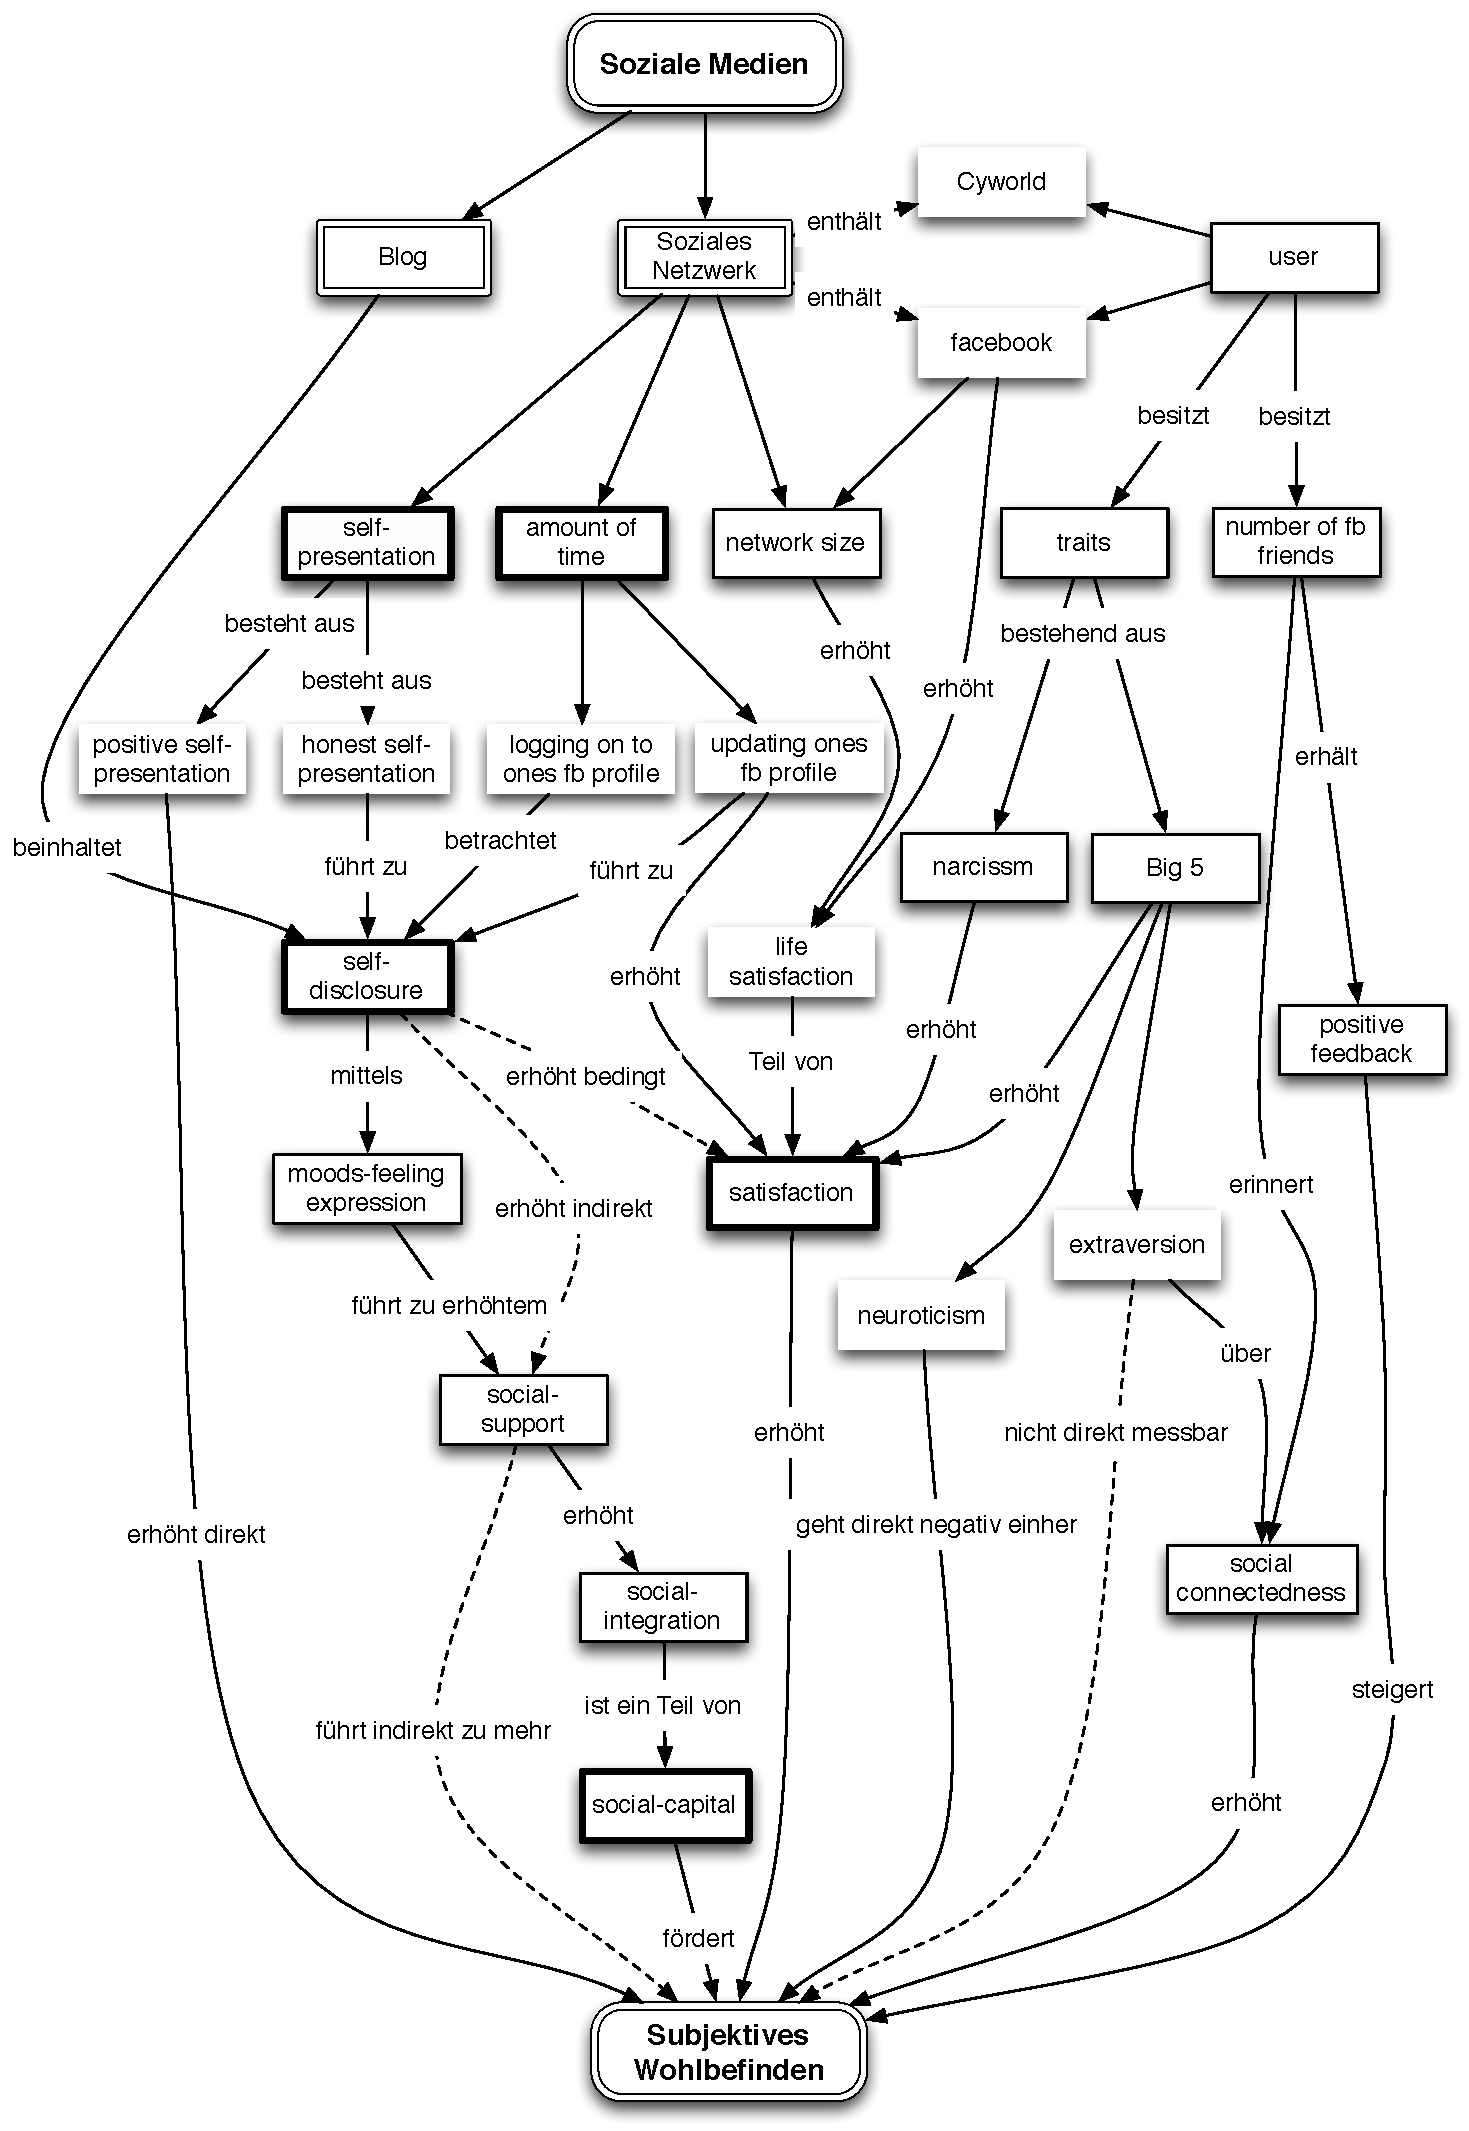
\includegraphics[width=0.9\textwidth]{images/grafiken/conceptMap_Swb_Sm_v2.pdf}
	\caption{ConceptMap - Subjektives Wohlbefinden und Soziale Medien}
	\label{fig.ConceptMapSwbSmAnhang}
\end{figure}



\end{document}
